\chapter{Utilizarea aplicației}
    \paragraph{} În acest capitol voi prezenta un exemplu de utilizare a aplicației pentru rularea unui server HTTP Apache (\textit{httpd}) și comenzile necesare pentru realizarea acestui lucru.

    \subsubsection{Pornirea daemonului}
        \paragraph{} Pentru pornirea daemonului se execută comanda \textbf{sudo minato -d}, care va porni programul în modul daemon și va începe să aștepte comenzi de la clienți.
        \begin{figure}[h!]
            \centering
            % \makebox[\textwidth][c]{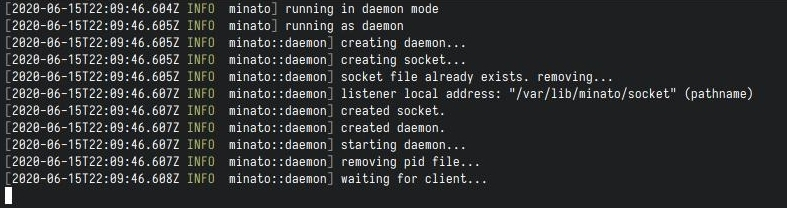
\includegraphics[width=1.2\textwidth]{daemon}}%
            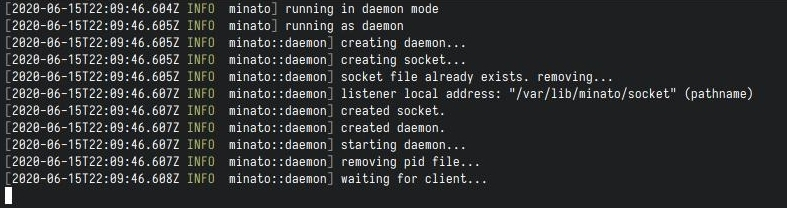
\includegraphics[width=1\textwidth]{daemon}
            \caption{Pornirea programului in modul daemon}
            \label{fig:daemon}
        \end{figure}

    \subsubsection{Downloadarea unei imagini}
        \paragraph{} Pentru downloadarea unei imagini se execută comanda \textbf{sudo minato -d image pull -i "alpine:latest"}. Aceasta va comunica cu daemonul și îi va trimite comanda pentru downloadarea unei imaginii a distributiei Alpine Linux. \textit{alpine} este id-ul folosit de imagine în Docker Hub, iar \textit{latest} este tag-ul acesteia, versiunea.
        \begin{figure}[h!]
            \centering
            % \makebox[\textwidth][c]{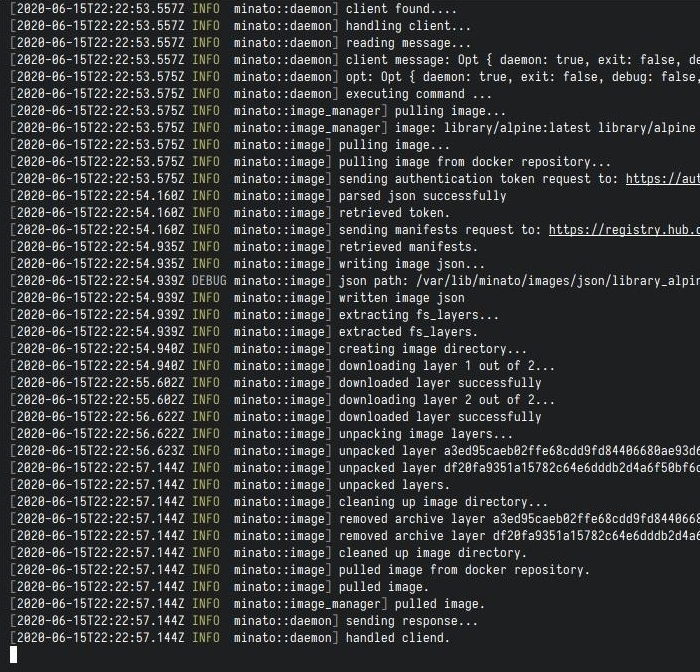
\includegraphics[width=1.25\textwidth]{pull}}%
            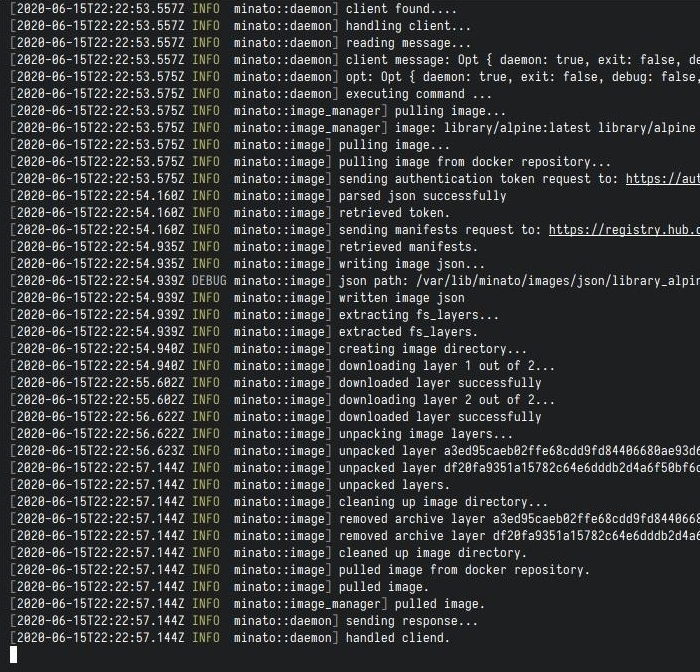
\includegraphics[width=1\textwidth]{pull}
            \caption{Downloadarea unei imagini}
            \label{fig:pull}
        \end{figure}

    \subsubsection{Crearea unui container}
        \paragraph{} Pentru crearea unui container se execută comanda \textbf{sudo minato -d container create -c "example" -i "alpine:latest"}. Aceasta va comunica cu daemonul și îi va trimite comanda pentru crearea unui container cu numele "example", folosind ca imagine distribuția Alpine Linux.

    \subsubsection{Listarea containerelor și a imaginilor}
        \paragraph{} Pentru listarea containerelor și a imaginilor se execută comanda \textbf{sudo minato container list}, respectiv \textbf{sudo minato image list}. În lista de containere sunt afișate numele, imaginea, locația și PID-ul (dacă acesta rulează) fiecărui container, iar in lista de imagini sunt afișate numele, versiunea și locația fiecărui container.
        \begin{figure}[h!]
            \centering
            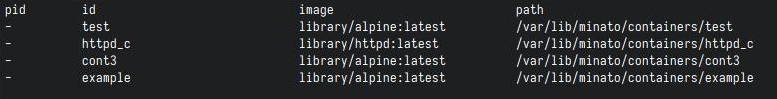
\includegraphics[width=1\textwidth]{clist}
            \caption{Listarea containerelor}
            \label{fig:clist}
        \end{figure}
        \begin{figure}[h!]
            \centering
            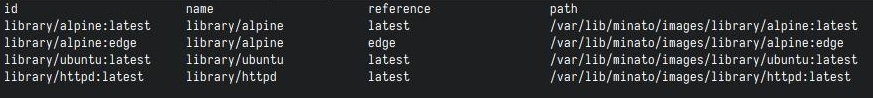
\includegraphics[width=1\textwidth]{ilist}
            \caption{Listarea imaginilor}
            \label{fig:ilist}
        \end{figure}

    \subsubsection{Rularea containerului}
        \paragraph{} Pentru rularea unui container se execută comanda \textbf{sudo minato -d container run -c example -v "/test:var/www/html"}. Aceasta va comunica cu daemonul și îi va trimite comanda pentru rularea containerului cu numele "example". De asemenea, se va crea o legătură (\textit{bind mount}) între directorul \textit{/test} din sistemul de operare gazdă și directorul \textit{/var/www/html} din container.
        \paragraph{} Odata ce primește comanda, daemonul va crea un proces nou, izolat față de restul sistemului de operare, apoi se va reîntoarce la starea de așteptare.
        \paragraph{} Pașii executați pentru rularea unui container sunt descriși în \autoref{section:run} și în figura \ref{fig:run}.

    \subsubsection{Deschiderea containerului}
        \paragraph{} Pentru deschiderea unui container se execută comanda \textbf{sudo minato container open -c example} într-un terminal separat. Programul va căuta apoi PID-ul containerului cu numele "example" și va crea un proces nou, un shell, în \textit{namespaceurile} acestuia.
        \begin{figure}[h!]
            \centering
            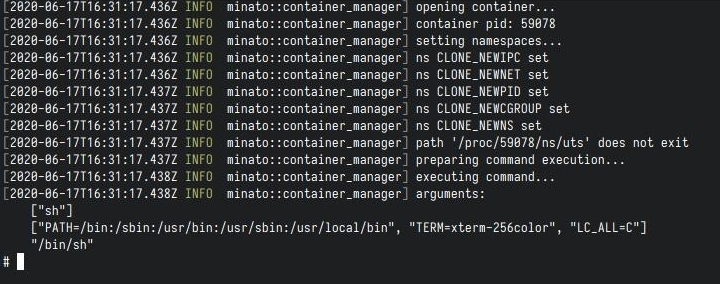
\includegraphics[width=1\textwidth]{open}
            \caption{Deschiderea unui container}
            \label{fig:open}
        \end{figure}

    \subsubsection{Instalarea și pornirea aplicației de server}
        \paragraph{} Odată deschis containerul, se instalează pachetele \textit{apache2}, aplicația pentru server, si \textit{openrc}, aplicația pentru servicii, folosind comanda \textbf{apt install apache2 openrc}. Pornirea serverului se face prin comanda \textbf{rc-service apache2 start}.
        \begin{figure}[h!]
            \centering
            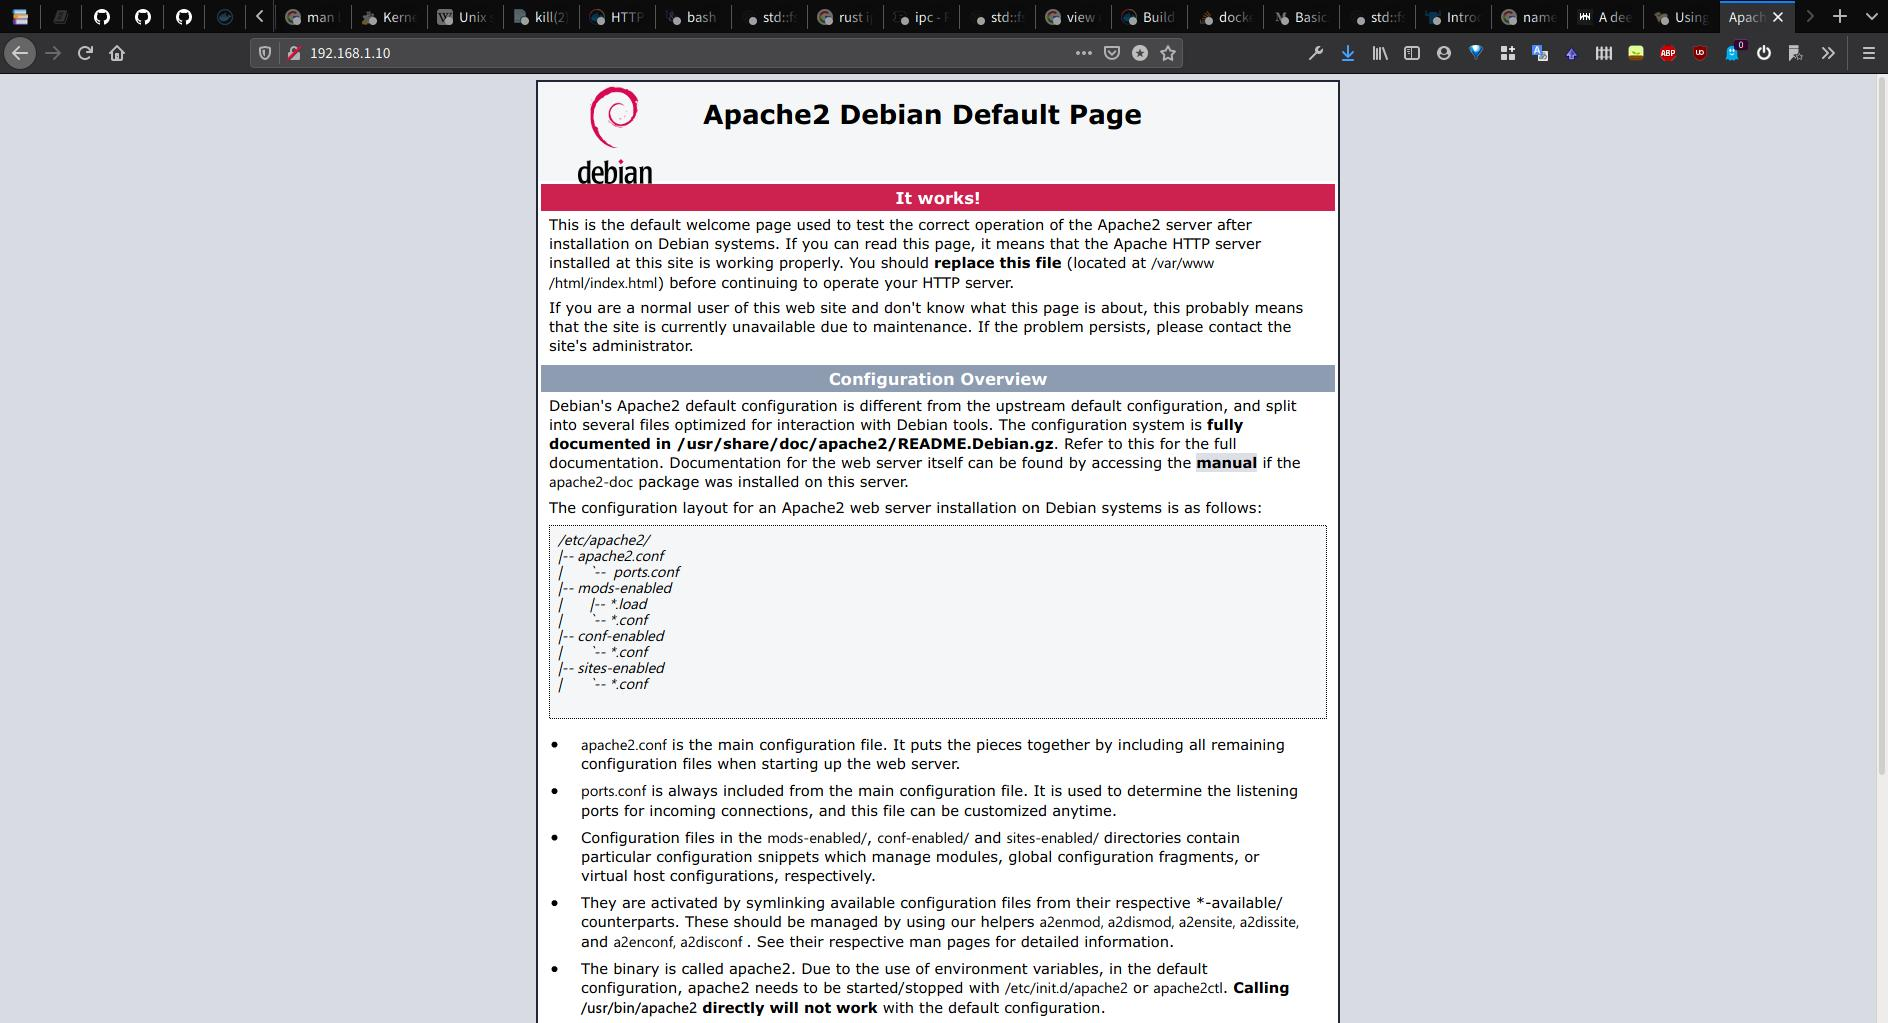
\includegraphics[width=1\textwidth]{apache2}
            \caption{Site-ul de start al serviciului httpd}
            \label{fig:apache2}
        \end{figure}
        \paragraph{} Fișierele site-ului hostat de server sunt stocate în \textit{/var/www/html} în container, dar sunt accesibile și din directorul \textit{/test} din sistemul de operare. De asemenea, site-ul poate fi vizualizat din sistemul de operare prin IP-ul \textbf{192.168.1.10}.
        \paragraph{} Această configurație permite rularea unui server sau a mai multor servere locale, fiecare asociat unui site și unui IP, și izolat față de celelalte.
        % fără a trebui să fie mutate fișierele.

    \subsubsection{Ștergerea containerului și a imaginii}
        \paragraph{} Odată ce containerul și imaginea nu mai sunt necesare, acestea pot fi șterse prin execuția comenzilor \textbf{sudo minato -d container delete -c example} și \textbf{sudo minato -d image delete -i "alpine:latest"}.

    \subsubsection{Oprirea daemonului}
        \paragraph{} Daemonul poate fi oprit prin execuția comenzii \textbf{sudo minato -e}.
